\documentclass[10pt, a4paper, oneside, notoc, nobib]{tufte-book} % Use the tufte-book class which in turn uses the tufte-common class


\hypersetup{colorlinks} % Comment this line if you don't wish to have colored links

\usepackage{microtype} % Improves character and word spacing

\usepackage{lipsum} % Inserts dummy text

\usepackage{booktabs} % Better horizontal rules in tables

\usepackage{graphicx} % Needed to insert images into the document
\graphicspath{{graphics/}} % Sets the default location of pictures
\setkeys{Gin}{width=\linewidth,totalheight=\textheight,keepaspectratio} % Improves figure scaling

\usepackage{fancyvrb} % Allows customization of verbatim environments
\fvset{fontsize=\normalsize} % The font size of all verbatim text can be changed here

\newcommand{\hangp}[1]{\makebox[0pt][r]{(}#1\makebox[0pt][l]{)}} % New command to create parentheses around text in tables which take up no horizontal space - this improves column spacing
\newcommand{\hangstar}{\makebox[0pt][l]{*}} % New command to create asterisks in tables which take up no horizontal space - this improves column spacing

\usepackage{xspace} % Used for printing a trailing space better than using a tilde (~) using the \xspace command

\newcommand{\monthyear}{\ifcase\month\or January\or February\or March\or April\or May\or June\or July\or August\or September\or October\or November\or December\fi\space\number\year} % A command to print the current month and year

\newcommand{\openepigraph}[2]{ % This block sets up a command for printing an epigraph with 2 arguments - the quote and the author
\begin{fullwidth}
\sffamily\large
\begin{doublespace}
\noindent\allcaps{#1}\\ % The quote
\noindent\allcaps{#2} % The author
\end{doublespace}
\end{fullwidth}
}

\newcommand{\blankpage}{\newpage\hbox{}\thispagestyle{empty}\newpage} % Command to insert a blank page

\usepackage{units} % Used for printing standard units

\newcommand{\hlred}[1]{\textcolor{Maroon}{#1}} % Print text in maroon
\newcommand{\hangleft}[1]{\makebox[0pt][r]{#1}} % Used for printing commands in the index, moves the slash left so the command name aligns with the rest of the text in the index 
\newcommand{\hairsp}{\hspace{1pt}} % Command to print a very short space
\newcommand{\ie}{\textit{i.\hairsp{}e.}\xspace} % Command to print i.e.
\newcommand{\eg}{\textit{e.\hairsp{}g.}\xspace} % Command to print e.g.
\newcommand{\na}{\quad--} % Used in tables for N/A cells
\newcommand{\measure}[3]{#1/#2$\times$\unit[#3]{pc}} % Typesets the font size, leading, and measure in the form of: 10/12x26 pc.
\newcommand{\tuftebs}{\symbol{'134}} % Command to print a backslash in tt type in OT1/T1

\providecommand{\XeLaTeX}{X\lower.5ex\hbox{\kern-0.15em\reflectbox{E}}\kern-0.1em\LaTeX}
\newcommand{\tXeLaTeX}{\XeLaTeX\index{XeLaTeX@\protect\XeLaTeX}} % Command to print the XeLaTeX logo while simultaneously adding the position to the index

\newcommand{\doccmdnoindex}[2][]{\texttt{\tuftebs#2}} % Command to print a command in texttt with a backslash of tt type without inserting the command into the index

\newcommand{\doccmddef}[2][]{\hlred{\texttt{\tuftebs#2}}\label{cmd:#2}\ifthenelse{\isempty{#1}} % Command to define a command in red and add it to the index
{ % If no package is specified, add the command to the index
\index{#2 command@\protect\hangleft{\texttt{\tuftebs}}\texttt{#2}}% Command name
}
{ % If a package is also specified as a second argument, add the command and package to the index
\index{#2 command@\protect\hangleft{\texttt{\tuftebs}}\texttt{#2} (\texttt{#1} package)}% Command name
\index{#1 package@\texttt{#1} package}\index{packages!#1@\texttt{#1}}% Package name
}}

\newcommand{\doccmd}[2][]{% Command to define a command and add it to the index
\texttt{\tuftebs#2}%
\ifthenelse{\isempty{#1}}% If no package is specified, add the command to the index
{%
\index{#2 command@\protect\hangleft{\texttt{\tuftebs}}\texttt{#2}}% Command name
}
{%
\index{#2 command@\protect\hangleft{\texttt{\tuftebs}}\texttt{#2} (\texttt{#1} package)}% Command name
\index{#1 package@\texttt{#1} package}\index{packages!#1@\texttt{#1}}% Package name
}}

% A bunch of new commands to print commands, arguments, environments, classes, etc within the text using the correct formatting
\newcommand{\docopt}[1]{\ensuremath{\langle}\textrm{\textit{#1}}\ensuremath{\rangle}}
\newcommand{\docarg}[1]{\textrm{\textit{#1}}}
\newenvironment{docspec}{\begin{quotation}\ttfamily\parskip0pt\parindent0pt\ignorespaces}{\end{quotation}}
\newcommand{\docenv}[1]{\texttt{#1}\index{#1 environment@\texttt{#1} environment}\index{environments!#1@\texttt{#1}}}
\newcommand{\docenvdef}[1]{\hlred{\texttt{#1}}\label{env:#1}\index{#1 environment@\texttt{#1} environment}\index{environments!#1@\texttt{#1}}}
\newcommand{\docpkg}[1]{\texttt{#1}\index{#1 package@\texttt{#1} package}\index{packages!#1@\texttt{#1}}}
\newcommand{\doccls}[1]{\texttt{#1}}
\newcommand{\docclsopt}[1]{\texttt{#1}\index{#1 class option@\texttt{#1} class option}\index{class options!#1@\texttt{#1}}}
\newcommand{\docclsoptdef}[1]{\hlred{\texttt{#1}}\label{clsopt:#1}\index{#1 class option@\texttt{#1} class option}\index{class options!#1@\texttt{#1}}}
\newcommand{\docmsg}[2]{\bigskip\begin{fullwidth}\noindent\ttfamily#1\end{fullwidth}\medskip\par\noindent#2}
\newcommand{\docfilehook}[2]{\texttt{#1}\index{file hooks!#2}\index{#1@\texttt{#1}}}
\newcommand{\doccounter}[1]{\texttt{#1}\index{#1 counter@\texttt{#1} counter}}

\usepackage{makeidx} % Used to generate the index
\makeindex % Generate the index which is printed at the end of the document

% This block contains a number of shortcuts used throughout the book
\newcommand{\vdqi}{\textit{VDQI}\xspace}
\newcommand{\ei}{\textit{EI}\xspace}
\newcommand{\ve}{\textit{VE}\xspace}
\newcommand{\be}{\textit{BE}\xspace}
\newcommand{\VDQI}{\textit{The Visual Display of Quantitative Information}\xspace}
\newcommand{\EI}{\textit{Envisioning Information}\xspace}
\newcommand{\VE}{\textit{Visual Explanations}\xspace}
\newcommand{\BE}{\textit{Beautiful Evidence}\xspace}
\newcommand{\TL}{Tufte-\LaTeX\xspace}




\setcounter{secnumdepth}{2}
\setcounter{tocdepth}{2}

\let\cleardoublepage\clearpage


\usepackage[utf8]{inputenc}
\usepackage{subfiles}
\usepackage{nameref}
\usepackage{lastpage}
\usepackage{physics}
\usepackage{amsmath}
\usepackage{pdfpages}
\usepackage{mwe}
\usepackage[sort&compress,numbers]{natbib}

% Command
\newcommand{\pfrac}[2]{\frac{\partial #1}{\partial #2}}
\newcommand{\pfracsquared}[2]{\frac{\partial^2 #1}{\partial #2^2}}
\newcommand{\unitary}[0]{\mathcal{U}}
\newcommand{\lindbladian}{\mathcal{L}}
\newcommand{\identity}{\mathbb{1}}

\newcommand{\fracsqrttwo}[0]{\frac{1}{\sqrt{2}}}

\DeclareMathOperator{\MVG}{MVG}
\DeclareMathOperator{\Uniform}{Uniform}
\DeclareMathOperator{\PDF}{PDF}
\DeclareMathOperator{\nLLH}{nLLH}
\DeclareMathOperator{\Var}{Var}
\DeclareMathOperator{\SNR}{SNR}


% \DeclareMathOperator{\erf}{erf}

% Colors 
% https://coolors.co/5f0f40-873b5e-af677c-ffbfb7-ffd447-48a9a6-243010
\definecolor{color1}{HTML}{5F0F40}
\definecolor{color2}{HTML}{873B5E}
\definecolor{color3}{HTML}{AF677C}
\definecolor{color4}{HTML}{ffbfb7}
\definecolor{color5}{HTML}{ffd447}
\definecolor{color6}{HTML}{48a9a6}
\definecolor{color7}{HTML}{243010}

\usepackage[color = color1, textcolor = white]{todonotes}

% Colors of stuff
\hypersetup{
    linkcolor = color6
}

%\renewcommand{\chaptermark}[1]{\markleft{\thechapter}}

% Header on pages
\fancypagestyle{fancy}{
  \fancyhf{} 
  \fancyhead[L]{\leftmark}
  \fancyhead[R]{\thepage}
}

% Header on Chapter Opening
\fancypagestyle{plain}{
  \fancyhf{} 
   \fancyfoot[R]{\thepage}
}

% chapter format
\titleformat{\chapter}%
  {\huge\bf\color{color1} }% format applied to label+text
  {\llap{\colorbox{color1}{\parbox{1.5cm}{\hfill\huge\bf\color{white}\thechapter}}\hspace{0.2cm}}}% label
  {0 cm}% horizontal separation between label and title body
  {}% before the title body
  []% after the title body

\titleformat{\section}%
  {\LARGE\bf\color{color2} }% format applied to label+text
  {\llap{\colorbox{color2}{\parbox{1.0cm}{\hfill\LARGE\bf\color{white}\thesection}}\hspace{0.2cm}}}% label
  {0 cm}% horizontal separation between label and title body
  {}% before the title body
  []% after the title body

\titleformat{\subsection}%
  {\bf\color{color3}}% format applied to label+text
  {\llap{{\hfill\bf\color{color3}\thesubsection}\hspace{0.2cm}}}% label
  {0 cm}% horizontal separation between label and title body
  {}% before the title body
  []% after the title body

\usepackage[pages=some]{background}
% Background picture of title page
\backgroundsetup{
    scale=1,
    color=black,
    opacity=0.4,
    angle=0,
    contents={%
      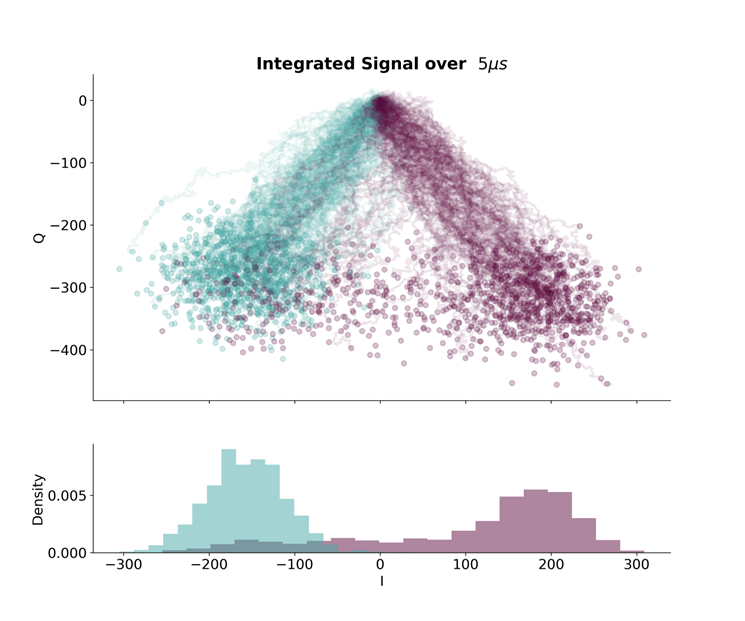
\includegraphics[width=\paperwidth,height=\paperheight]{Figs/Theory/stochastic_signal.png}
      }%
}